\documentclass[12pt,letterpaper]{hmcpset}
\usepackage[margin=1in]{geometry}
\usepackage{graphicx}
\usepackage{enumitem} % enumerate
\newcommand{\vb}{\mathbf}
% example usage of amssymb: $\mathbb{Z}$
% amsmath is loaded.

% info for header block in upper right hand corner
\name{}
\class{Math 19 - \phantom{07}}
\assignment{Homework \#10}
\duedate{11/8/2019}

\begin{document}

\problemlist{Colley 2.5.4, 2.5.10, 2.5.22, 2.5.36, \\ 2.6.5, 2.6.11, 2.6.12, 2.6.13, 2.6.16}

\begin{problem}[Colley 2.5.4]
  Suppose that $z = x^2 + y^3$, where $x = st$ and $y$ is a function of $s$ and $t$.
  Suppose further that when $(s,t) = (2,1),~\partial y/\partial t = 0$.
  Determine $\displaystyle \frac{\partial z}{\partial t}(2, 1)$.
\end{problem}
\clearpage

\begin{problem}[Colley 2.5.10]
  A clarinetist is playing the glissando at the beginning of
  \textit{Rhapsody in Blue}, while Hermione (who arrived late)
  is walking toward her seat.
  If the (changing) frequency of the note is $f$ and Hermione is moving toward the clarinetist at speed $v$, then she actually hears the frequency $\phi$ given by
  \[ \phi = \frac{c + v}{c}f, \]
  where $c$ is the (constant) speed of sound in air, about 330m/sec.
  At this particular moment, the frequency is $f = 440$ Hz and is increasing at a rate of 100 Hz per second.
  At that same moment, Hermione is moving toward the clarinetist at 4 m/sec and decelerating at 2 m/sec$^2$.
  What is the percieved frequency $\phi$ she hears at that moment?
  How fast is it changing?
  Does Hermione hear the clarinet's note becoming higher or lower?
\end{problem}
\clearpage

\begin{problem}[Colley 2.5.22]
  Calculate $D(\vb f \circ \vb g)$ in two ways:
  (a) by first evaluating $\vb f \circ \vb g$ and
  (b) by using the chain rule and the derivative matricies $D\vb f$ and $D\vb g$.
  \[ f(x,y) = x^2 - 3y^2,~\vb g(s, t) = (st, s+t^2) \]
\end{problem}
\clearpage

\begin{problem}[Colley 2.5.36]
  Suppose that you are given an equation of the form
  \[ F(x,y,z) = 0, \]
  for example, something like $x^3z + y\cos z + (\sin y)/z = 0$.
  Then we may consider $z$ to be defined implicitly as a function $z(x, y)$.
  \begin{enumerate}[label=(\alph*)]
  \item Use the chain rule to show that if $F$ and $z(x,y)$ are both assumed to be differentiable, then
    \[\frac{\partial z}{\partial x} = -\frac{F_x(x,y,z)}{F_z(x,y,z)},\qquad \frac{\partial z}{\partial y} = -\frac{F_y(x,y,z)}{F_z(x,y,z)} \]
  \item Use part (a) to find $\partial z/\partial x$ and $\partial z / \partial y$ where $z$ is given by the equation $xyz = 2$.
    Check your result by explicitly solving for $z$ and then calculating the partial derivatives.
  \end{enumerate}
\end{problem}
\clearpage

\begin{problem}[Colley 2.6.5]
  Calculate the directional derivative of the given function $f$ at the point $\vb a$ in the direction parallel to the vector $\vb u$.
  \[ f(x, y) = e^x - x^2y,\quad\vb a = (1, 2),\quad\vb u = 2\vb i + \vb j \]
\end{problem}
\clearpage

\begin{problem}[Colley 2.6.11]
  The surface of Lake Erehwon can be represented by a region $D$ in the $xy$-plane such that the lake’s depth (in meters) at the point $(x, y)$ is given by the expression $400 - 3x^2y^2$.
  If your calculus instructor is in the water at the point $(1, -2)$, in which direction should she swim
  \begin{enumerate}[label=(\alph*)]
  \item so that the depth increases most rapidly (i.e., so that she is most likely to drown)?
  \item so that the depth remains constant?
  \end{enumerate}
\end{problem}
\clearpage

\begin{problem}[Colley 2.6.12]
  A ladybug (who is very sensitive to temperature) is crawling on graph paper.
  She is at the point $(3, 7)$ and notices that if she moves in the $\vb i$-direction, the temperature \textit{increases} at a rate of 3 deg/cm.
  If she moves in the $\vb j$-direction, she find that her temperature \textit{decreases} at a rate of 2 deg/cm.
  In what direction should the ladybug move if
  \begin{enumerate}[label=(\alph*)]
  \item she wants to warm up most rapidly?
  \item she wants to cool off most rapidly?
  \item she desires her temperature \textit{not} to change?
  \end{enumerate}
\end{problem}
\clearpage

\begin{problem}[Colley 2.6.13]
  You are atop Mt. Gradient, 5000 ft above sea level, equipped with the topographic map shown in Figure 2.74.
  A storm suddenly begins to blow, necessitating your immediate return home.
  If you begin heading due east from the top of the mountain, sketch the path that will take you down to sea level most rapidly.
\end{problem}
  \begin{figure}[ht]
    \centering
    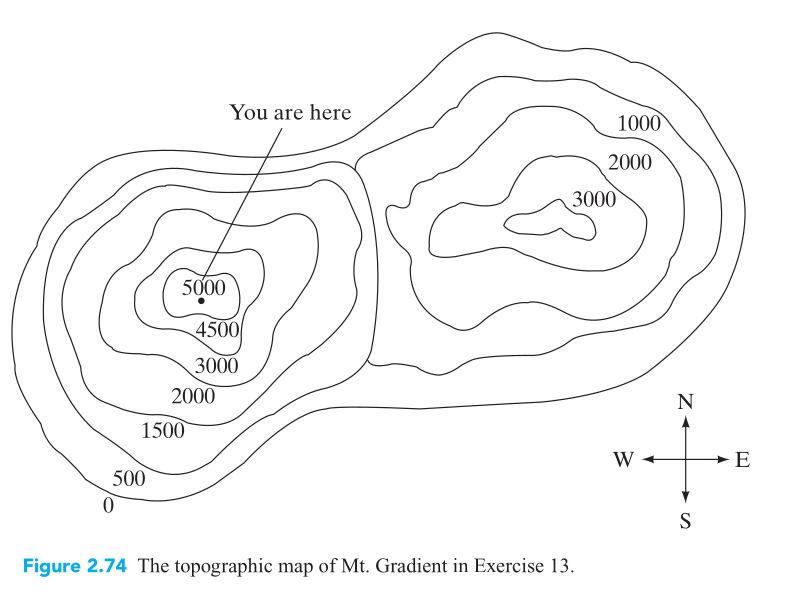
\includegraphics[width=\textwidth]{assets/10_map.png}
  \end{figure}
\clearpage

\begin{problem}[Colley 2.6.16]
  Find an equation for the tangent plane to the surface given by the equation at the indicated point $(x_0, y_0, z_0)$.
  \[ x^3 + y^3 + z^3 = 7,\quad (x_0, y_0, z_0) = (0, -1, 2) \]
\end{problem}

\end{document}
